\documentclass[12pt]{article}

\usepackage[margin=0.5in]{geometry}
\usepackage{amsmath}
\usepackage{tikz}
\usepackage{hyperref}
\usepackage{soul}
\usepackage{multicol}

\newcommand{\ds}{\displaystyle}

\begin{document}
\pagestyle{empty}
\subsubsection*{Midterm 3 Review Problems \hfill Math 140 }
\textit{These are suggested review problems similar to what might be on Midterm 3. Included with each problem is a link to a video where you can see how the problem is solved. I didn't make the videos.}

\begin{enumerate}


\item Find the absolute max and min for $f(x) = x^3 - 3x^2$, $-\frac{1}{2} \le x \le 4$. 
\vfill 
\hfill  \url{https://youtu.be/S3YA6K9iEGM}
\hrule 

\item Find the intervals of increase \& decrease for the function $f(x) = 2x^3+18x^2+30x+3$.
\vfill
\hfill \url{https://youtu.be/jB451pFTi6c}
\hrule

\item Determine the increasing \& decreasing intervals for $f(x) = \dfrac{x}{x^2+1}$.  
\vfill
\hfill \url{https://youtu.be/oThEqQVHo9c}
\hrule

\item Find the intervals of increase/decrease for $f(x) = (x^2-1)^3$.
\vfill
\hfill \url{https://youtu.be/jJb_Qk0O5a0?t=263}
\hrule


\item Morpheus sells 1000 packages of sleeping pills every month at a price of \$12 per package. Suppose that for each \$1 increase in price, 10 less packages would be sold. At what price should Morpheus sell each package in order to maximize his revenue?
\vfill
\hfill \url{https://youtu.be/vfIFLryA_DU}
\hrule


\newpage
\item Find the dimensions of the rectangle with largest area when its base lies on the x-axis and its two top corners are on the parabola $y = 8 - x^2$. 
\begin{flushright}
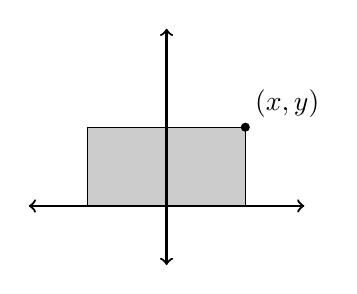
\begin{tikzpicture}[scale=0.5]
\filldraw[fill=gray!40] (-2,0) rectangle (2,2);
\draw[thick,<->] (-3.5,0) -- (3.5,0);
\draw[thick,<->] (0,-1.5) -- (0,4.5);
\draw[very thick,color=blue] plot[domain=-3:3,samples=400] function {(8-x**2)/2};
\filldraw (2,2) circle (0.1) node[above right] {$(x,y)$};
\end{tikzpicture}
\end{flushright}
\hfill \url{https://youtu.be/EOJbmMB8uCQ}
\hrule


\item Find the differential of $y = \sqrt{x}$ at $x = 16$ when $dx = 4$ Use it to approximate $\sqrt{20}$. 
\vfill
\hfill \url{https://youtu.be/0jG3enZdEmk}
\hrule


\item Suppose that a company has demand function $Q(p) = 10 - \frac{1}{2}p$ where $p$ is price.  Calculate the price elasiticty of demand when $p = \$16$. Recall that $E = \left| \dfrac{pQ'}{Q} \right|$. 
\vfill
\hfill \url{https://youtu.be/io4GwFGiVcI?t=446}
\hrule

\item Find the differential $dy$ for each of the following functions. 
\begin{enumerate}
\item $y = x^3 - 5 x + 10$ at $x = 2$ when $dx = \tfrac{1}{4}$. \\ \bigskip
\item $y = 2x^3 - 4x^2 + 8x - 1$ at $ x= 3$ when $dx = 0.1$.
\end{enumerate}
\vfill
\hfill \url{https://youtu.be/C5RI5eLzVfo?t=78}
\hrule



\newpage

\item Find the intervals where $f(x) = 2+3x^2 - x^3$ is concave up and the intervals where it is concave down.  Also, find the inflection points of $f(x)$.  
\vfill
\hfill \url{https://youtu.be/c1N8zyVhWxM}
\hrule

\item Find the intervals where $h(x) = (x^2-1)^3$ is concave up and the intervals where it is concave down.
% NOTE TO SELF: THIS ONE IS REALLY TOO HARD!!!  
\vfill
\hfill \url{https://youtu.be/c1N8zyVhWxM?t=183}
\hrule

\item If a stereo manufacturer wants to sell $x$ units of a new stereo, the price per unit (in dollars) must be 
$$p(x) = 1000 - x.$$
The total cost of producing $x$ stereos is 
$$C(x) = 3000 + 20x.$$
Find the level of production $x$ that maximizes profit. Recall that profit is revenue minus cost and revenue is price times quantity sold. 

\vfill
\hfill \url{https://www.youtube.com/watch?v=XEr-t6TWP18&t=19s}
\hrule


\item Find the partial derivatives $\dfrac{\partial z}{\partial x}$ and $\dfrac{\partial z}{\partial y}$ for the function $z= e^{x^2 y^3}.$
%\begin{enumerate}
%\part $f(x,y) = 7x^2 - x^3 y^4 + 5x^4 y^3
%
%\end{enumerate}

\vfill
\hfill \url{https://youtu.be/JAf_aSIJryg?t=311}
\hrule

\end{enumerate}
\end{document}
